  \section[Resource Description Framework (RDF)]{RDF}
  \label{sec:rdf}

  \initial{R}\textit{esource Description Framework (RDF)}\
  is a World Wide Web Consortium (W3C) standardized data model for representing\
  semantic Web resources. It uses graphs to represent information using a triple-based\
  notation comprising a subject, predicate and an object. All these entities\
  can be uniquely identified by Internationalized Resource Identifiers\
  (IRIs)~\citep{pathak_applying_2012}.

  \subsection{How we can use it}

  We can use it by evoking already existing tools such as D2R Map \citep{_d2r_tool_2013}\
  which is an open source tool thats transfers relational data into RDF\
  format which will then allow us to easily gain better insight between data.\

  \subsection{Why this model would be useful for our application}

  RDF offers a practical evolutionary pathway to semantic interoperability.\
  It enables information to be readily linked and exchanged with full semantic\
  fidelity while leveraging existing IT infrastructure investments.\
  Being schema-flexible, RDF allows multiple evolving data models and vocabularies\
  to peacefully co-exist in the same instance data, without loss of semantic fidelity.\
  This enables standardized data models and vocabularies to be used whenever possible,\ 
  while permitting legacy or specialized models and vocabularies to be\
  semantically linked and used when necessary. It also enables a limitless\
  variety of related information to be semantically linked to patient data,\
  such as genomic, geographic and drug interaction data, enabling more effective\
  treatment, and greater knowledge discovery. Other reasons for adopting RDF as\
  a universal healthcare exchange language include~\citep{_Munnecke_2013}:
  \begin{itemize}
    \itemsep0ex
    \item Its ability to make information self-describing with precise semantics
    \item Its support for automated inference
    \item Its foundation in open standard
  \end{itemize}

  \noindent By using a standard language for data interchange, new research discoveries could be made\
  more efficiently and effectively.\

  \subsection{RDF Examples}
  \begin{figure}[h!]
    \begin{subfigure}[b]{.5\linewidth}
      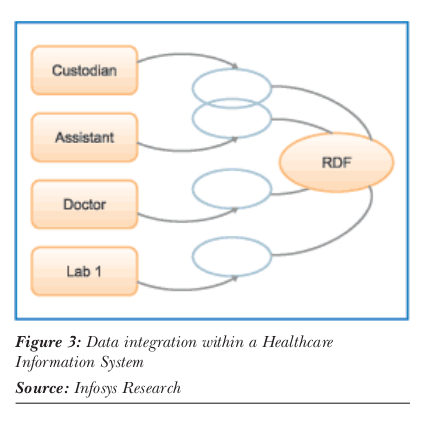
\includegraphics[width=1.0\textwidth]{rdfh.png}
      \caption{RDF Example 1}
      \label{fig:third}
    \end{subfigure}
    ~
    \begin{subfigure}[b]{.5\linewidth}
      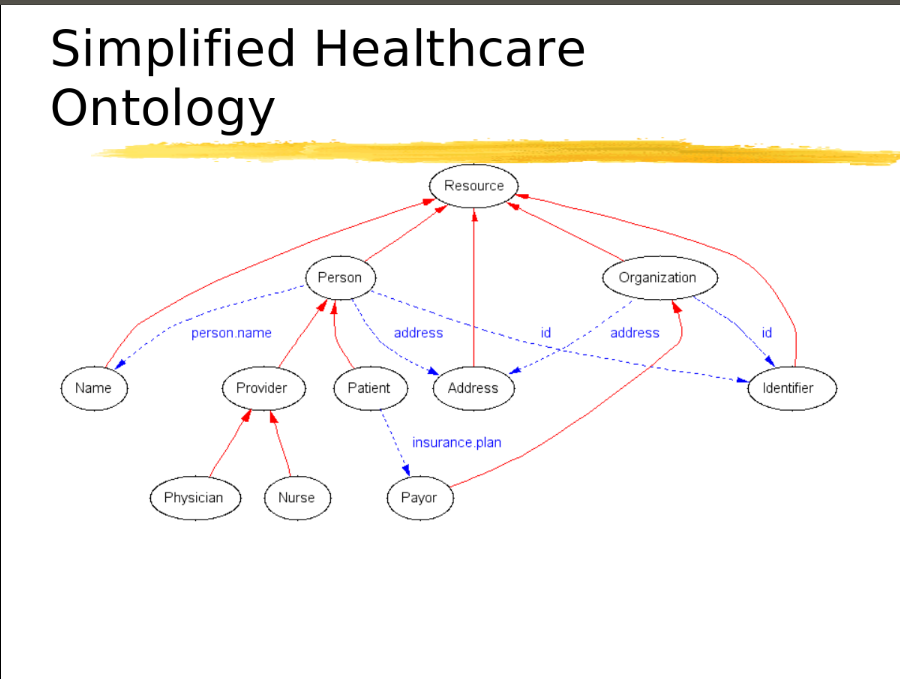
\includegraphics[trim=4 1 1 7,clip,width=\textwidth]{rdf1.png}
      \caption{RDF Example 2}
      \label{fig:fourth}
    \end{subfigure}
    \caption{Examples}
    \label{fig:rdf_examples}
  \end{figure}

  \noindent The first and second subfigures in subfigure\
  2 are labeled as\
  \ref{fig:third} \citep{parachuri2008role}\
  and~\ref{fig:fourth}~\citep{_Borden_2013} respectively.\\


 \subsection{Comparison with other data models}

  \begin{figure}[ht!]
    \centering
    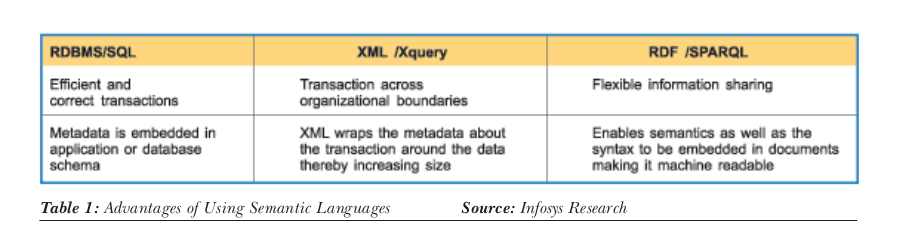
\includegraphics[scale=0.5]{sqlrdf.png}
    \caption{Comparison of RDF, XML and SQL}
    \citep[Fig.~1]{parachuri2008role}
    \label{fig:nwhin}
  \end{figure}  

  \subsubsection{XML}
  XML is a comparable data model to RDF and in fact one way you can express RDF data is in a certain XML format.\
  What sets RDF apart from XML is that RDF is designed to represent knowledge in a distributed world.\
  That RDF is designed for knowledge, and not data, means RDF is particularly concerned with meaning.\\

  \noindent In some ways, RDF can be compared to XML. XML also is designed to be simple and applicable to any type of data.\
  XML is also more than a file format. It is a foundation for dealing with hierarchical, self-contained documents,\
  whether they be stored on disk in the usual brackets-and-slashes format, or held in memory and accessed through a DOM API.\
  \citep{_rdf_about_2013}\

  \subsubsection{SQL}
  Relational Database’s such as SQL is also a comparable data model to RDF, and\
  you can actually store your RDF data inside of a relational database.\
  Individual statements in RDF are expressed as subject, predicate, object\ 
  triples. Sets of these with a common predicate can be mapped to binary relations\
  in the relational model, in the the common parlance, 2-column tables.\\

  \noindent But a difference between the two is that in Relational DB's, for a certain\
  set of values a relation is either considered either true (there is a corresponding\
  row in the table) or false (there isn't). In the RDF model in the general case,\
  if a set of values isn't in the ``row'' (i.e. you don't have a particular statement),\
  then it's not false, just unknown. \citep{_rdf_comparison_2013}\
